%!TEX root = ../main.tex
% Chapter 10

\chapter{Nutzerbefragung zum Bezahl- und Tokensystem}
\label{Nutzerbefragung_zum Bezahl-_und_Tokensystem}
Das folgende Kapitel beschreibt die Konzeption und Durchführung einer nicht repräsentativen Umfrage zum Bezahl- und Tokensystem auf Basis des Prototyps aus Kapitel \ref{Implementation_eines_Prototyps_zum Bezahl-_und_Tokensystem}. Im Gegensatz zu einer detaillierten Systemevaluation soll die Befragung eine möglichst große Zahl an Antworten ergeben, wie in Kapitel \ref{Vorgehensweise} erläutert. Die Ergebnisse der Befragung dienen als Grundlage für die Auswahl des Bezahl- und Tokensystems.

\section{Konzeption der Befragung}
Die Befragung wird zweiteilig gestaltet. Zu Beginn wird der Prototyp unter \\ \url{https://proto.pay2mail.org/send} vorgestellt. Die Teilnehmer haben die Möglichkeit eigenständig durch den Prototypen zu navigieren, ihnen wird dabei die Aufgabe gestellt eine dringende E-Mail zu versenden. Da sie das hohe Aufkommen des Empfängers sehen werden, sind sie aufgefordert die Zahlung zu tätigen. Dafür wird ein Betrag ausgewählt und abgesendet, ohne eine wirkliche Zahlung zu vollziehen. Den Teilnehmern wird bewusst keine Auswahl an Zahlungsmethoden oder Tokensystemen gegeben. So können sie sich mit dem System vertraut machen und die für sie durch Online-Shops bekannteste Form des Gegenwertes, also Echtgeld, nutzen.

Nachdem sie den Prototypen genutzt haben, werden den Teilnehmern vier Fragen gestellt. Zu Beginn wird gefragt, welches System zur Priorisierung der Teilnehmer bevorzugt: Zahlung mit Echtgeld, Zahlung mit vorher ausgehändigten Token oder Verbot von Zahlungen zur Priorisierung. Obwohl letztere Option das Problem der Priorisierung aus Kapitel \ref{Problemfeld_und_Folgen} nicht lösen würde, wurde sie trotzdem in die Befragung eingebunden, um eine mögliche Nutzerakzeptanz des späteren Systems erahnen zu können. Würde sich eine große Zahl an Teilnehmer gegen eine Zahlung im Generellen entscheiden, würde dies die Frage aufwerfen inwieweit Pay2Mail genutzt werden würde. Die restlichen Fragen beziehen sich auf Stamminformationen der Teilnehmer: Alter, Geschlecht und Jahresbruttoeinkommen. Diese Stamminformationen haben keinen direkten Bezug zum Bezahlsystem, geben aber die Möglichkeit Schlussfolgerungen zu ziehen und die Ergebnisse im Kontext zu betrachten. 

Während der Nutzung des Prototyps und der Befragung werden die Teilnehmer in Präsenz beaufsichtigt, um aufkommende Fragen zu klären. Daher wird die Befragung mündlich durchgeführt, die Ergebnisse werden notiert. So können sich die Teilnehmer auf den Prototypen und das Bezahlsystem fokussieren.

Die Teilnehmer werden über soziale Medien, Unternehmen und dem erweiterten Bekanntenkreis so zusammengesetzt, dass sie eine möglichst heterogene Menge hinsichtlich ihrer Stamminformationen ergeben. Außerdem wird bei der Auswahl der Teilnehmer auf einen souveränen und häufigen E-Mail Verkehr geachtet. So wird vermieden, dass Teilnehmer befragt werden, die mit E-Mails selten in Kontakt kommen und kein Interesse an der Thematik haben. Die Souveränität im Umgang mit E-Mails ist erforderlich, damit die Teilnehmer bereits mit der Problematik von Triage und Priorisierung vertraut sind und die Ineffizienz des E-Mail Standardheaders \textit{Priority} kennen.

\section{Ergebnisse der Befragung}
\label{Ergebnisse_der_Befragung}
Es wurden 39 Personen im Alter von 18 bis 62 und einem Jahresbruttoeinkommen von 900€ bis 105.000€ befragt. Davon haben 17 angegeben, dass sie männlich und 18 angegeben, dass sie weiblich sind. 4 Personen machten zu ihrem Geschlecht keine Angabe. Die vollständigen Rohdaten der Befragung sind in Anhang \ref{tab:rohdaten} zu finden.

Die Mehrheit der Befragten (61,5\%) entschied sich dabei für ein Zahlungssystem mit Echtgeld, während sich 23,1\% für ein Tokensystem und 15,4\% gegen eine Zahlung im Allgemeinen aussprachen. Allerdings lassen sich große Unterschiede je nach Einkommen feststellen, wie in Abbildung \ref{fig:Auswahl_des_Zahlungssystems_der_Befragten_nach_Jahresbruttoeinkommen} zu sehen. So gibt es in der Gruppe der Jahresbruttoeinkommen kleiner als 20.000€ keine Mehrheit für ein System, stattdessen sind die Stimmen gleich verteilt. In der Gruppe der Einkommen zwischen 20.000€ und 40.000€ findet sich eine ähnliche Verteilung wie in der Gesamtzahl der Stimmen mit 66,7\% für Echtgeld, 25\% für Token und 8,3\% gegen ein Zahlungssystem. In der darauf folgenden Gruppe der Einkommen (40.000€ bis 60.000€) verändert sich die Verteilung stark zugunsten der Zahlung mit Echtgeld. Diese erreicht mit 81,8\% einen Höchstwert, während Zahlungen mit Token und die Ablehnung der Zahlung (jeweils 9,1\%) deutlich weniger Befragte überzeugen.

\begin{figure}[!ht]
\centering
\caption[Ergebnisse der Befragung nach Jahresbruttoeinkommen]{Ergebnisse der Befragung nach Jahresbruttoeinkommen}
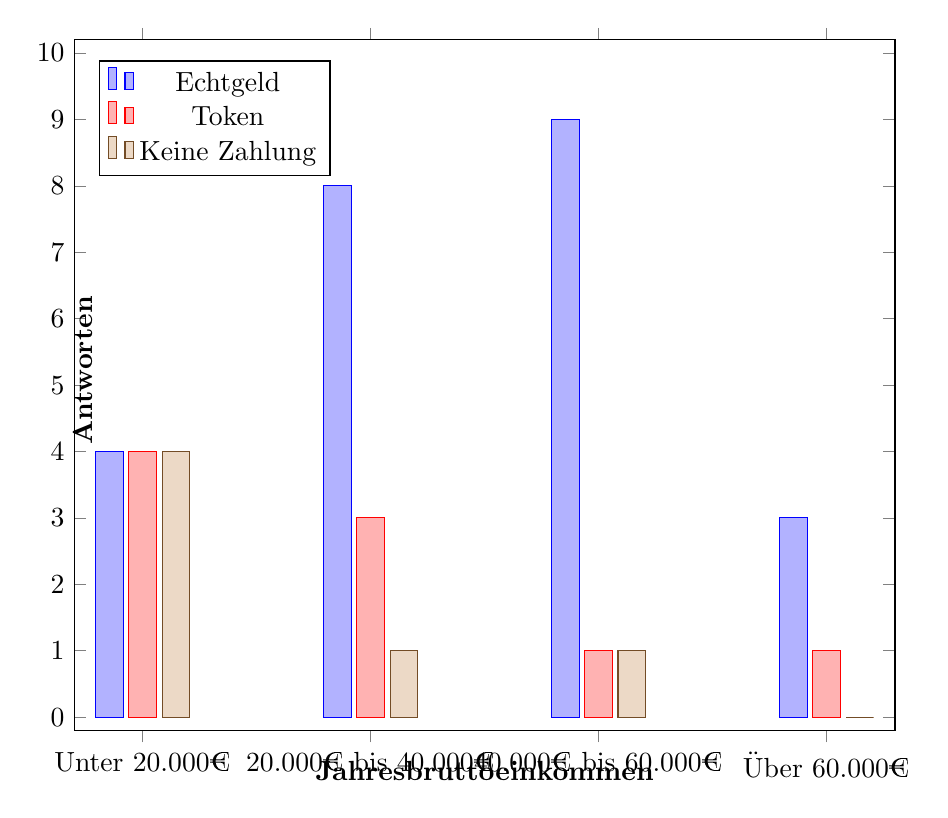
\begin{tikzpicture}
    \begin{axis}[
        ybar,
        ymin=0,ymax=10,
        x label style={at={(axis description cs:0.5,-0.03)},anchor=north},
        y label style={at={(axis description cs:0.01,0.4)},anchor=west},
        ylabel= \textbf{Antworten},
        xlabel= \textbf{Jahresbruttoeinkommen},
        enlarge x limits  = 0.1,
        enlarge y limits  = 0.02,
        symbolic x coords={Unter 20.000€,20.000€ bis 40.000€,40.000€ bis 60.000€,Über 60.000€},
        xtick=data,
        width=0.99\textwidth,
        legend pos=north west
    ]
    \addplot coordinates
    {(Unter 20.000€, 4) (20.000€ bis 40.000€, 8) (40.000€ bis 60.000€, 9) (Über 60.000€, 3)};
    \addplot coordinates
    {(Unter 20.000€, 4) (20.000€ bis 40.000€, 3) (40.000€ bis 60.000€, 1) (Über 60.000€, 1)};
    \addplot coordinates
    {(Unter 20.000€, 4) (20.000€ bis 40.000€, 1) (40.000€ bis 60.000€, 1) (Über 60.000€, 0)};
    \legend{Echtgeld, Token, Keine Zahlung}
    \end{axis}
\end{tikzpicture}
\label{fig:Auswahl_des_Zahlungssystems_der_Befragten_nach_Jahresbruttoeinkommen}
\end{figure}

Diese drei Gruppen können miteinander verglichen werden, da sie in ähnlicher Häufigkeit in der Befragung vorkommen (jeweils 12, 12 und 11 Befragte). Die Gruppe der Einkommen größer als 60.000€ lässt sich hingegen nicht vergleichen, da hier lediglich vier Angaben vorliegen. Allerdings gibt es in dieser Gruppe nur eine Stimme gegen Echtgeld.

Aus den Daten lässt sich schlussfolgern, dass die Bereitschaft für eine Priorisierung zu zahlen, insbesondere mit Echtgeld, steigt je höher das eigene Einkommen ist. Das bedeutet allerdings auch, dass Personen mit einem niedrigeren Einkommen bei der Nutzung von Pay2Mail potenziell benachteiligt werden. Diese Problematik wird in Kapitel \ref{Schluss} näher behandelt. 

Hinsichtlich Geschlecht lassen sich keine weiteren Schlüsse ziehen. Die Ergebnisse von männlichen und weiblichen Befragten (64,7\% und 66,7\% für Echtgeld; 23,5\% und 22,2\% für Token; 11,8\% und 11,1\% gegen Zahlungen) ähneln den Gesamtergebnissen, siehe Abbildung \ref{fig:Ergebnisse_der_Befragung_nach_Geschlecht}. Die Anzahl der Befragten ohne Angabe des Geschlechts beläuft sich auf vier, was keine tragfähigen Aussagen zulässt. Auch bezogen auf das Alter der Befragten lassen sich keine weiteren Schlüsse folgern, siehe Abbildung \ref{fig:Ergebnisse_der_Befragung_nach_Alter}. In jeder Altersklasse, in Zehnjahresstufen unterteilt, überwiegt Echtgeld als bevorzugtes Zahlungssystem. Der niedrigste Zustimmungswert ist dabei 42,9\% in der Gruppe der 20- bis 30-Jährigen; der höchste Zustimmungswert ist 100\% in der Gruppe der über 60-Jährigen, wobei hier nur zwei Stimmen gezählt wurden. Die Ergebnisse für Echtgeld sind auch in den Gruppen der 30- bis 40-Jährigen (85,7\%) und 50- bis 60-Jährigen (87,5\%) sehr hoch.

\section{Auswahl eines Bezahl- und Tokensystems}
\label{Auswahl_eines_Bezahl-_und_Tokensystems}
Die Mehrheit der Befragten entschied sich in der Umfrage für ein Bezahlsystem mit Echtgeld. Die Entscheidung war über alle anhand von Geschlecht, Alter und Einkommen relevanten klassifizierten Gruppen eindeutig. 

Die einzige Ausnahme ist die Gruppe der Jahresbruttoeinkommen unter 20.000€, welche keine Mehrheiten aufweist. In der Befragung gaben 12 der 39 Teilnehmer an, dass sie unter 20.000€ im Jahr netto verdienen, was etwa 31\% der Gesamtmenge der Befragten entspricht. Im Gegensatz dazu ergab eine Stichprobe des statistischen Bundesamtes, dass lediglich 17,8\% der von ihnen befragten Personen ein Jahresbruttoeinkommen von unter 20.000€ haben \citep[S. 25 f.]{StatistischesBundesamt2018}. Das lässt darauf schließen, dass der Anteil in der durchgeführten Umfrage unverhältnismäßig groß war im Vergleich zur Stichprobe des statistischen Bundesamtes.

Unter diesem Gesichtspunkt ist es vertretbar Echtgeld als Zahlungsform von Pay2Mail zu nutzen. Allerdings sollte nach Einführung des Systems geprüft werden, inwiefern Personen mit geringerem Einkommen benachteiligt werden. Nach der Implementation und Evaluation des Systems wird die Frage der sozialen Gerechtigkeit bei der Priorisierung von E-Mails in Kapitel \ref{Reflektion_und_Bewertung} weiter thematisiert. 
